\newpage 
\section{Annotated Designs}
In this section, three potential designs for each of the main pages of the application have been included, as well as annotations which link design decisions to the functional requirements. These designs focus on the landing page (which doubles as the route discovery page), the route creation page, the route listing page, and a single design for the route creation page. The other pages of the application are simple form pages, and do not need much thought, thus they have been included separately in section \ref{subsec:gpd}, along with some annotations. 

\subsection{The Landing Page/Route Discovery Page}
The purpose of the landing page (which doubles as the route discovery page), is to allow the user's for look for routes they may be interested. This is achieved by some search functionality, with the ability to specify extra filters if the user wishes (FR 1). 

\paragraph{Minimal Design}\ \\
The main driving idea behind the first design, is simplicity. It should be clear to the user, at all points, what they can do and what their next steps should be. This design sports a large map which, if possible, displays the user's current location in the background. This helps the user feel more acquainted with the application, because it is showing familiar surroundings - this is also the reason for displaying the ``Welcome, \textit{name}'' message by the search bar (although it will show ``explorer'' instead of the user's name if they are not logged in).\ \\
\ \\
To keep the page looking as clean as possible, the extra filter options are initially hidden (this includes price of petrol, distance travel, etc). This means users are able to search for routes, without being bombarded with a large number of form elements. This clean design and low number of elements on the page, make it very easy for the user to identify what this page's purpose is - searching for routes.
\begin{figure}[!ht]
\vspace{6mm}
 \begin{center}
		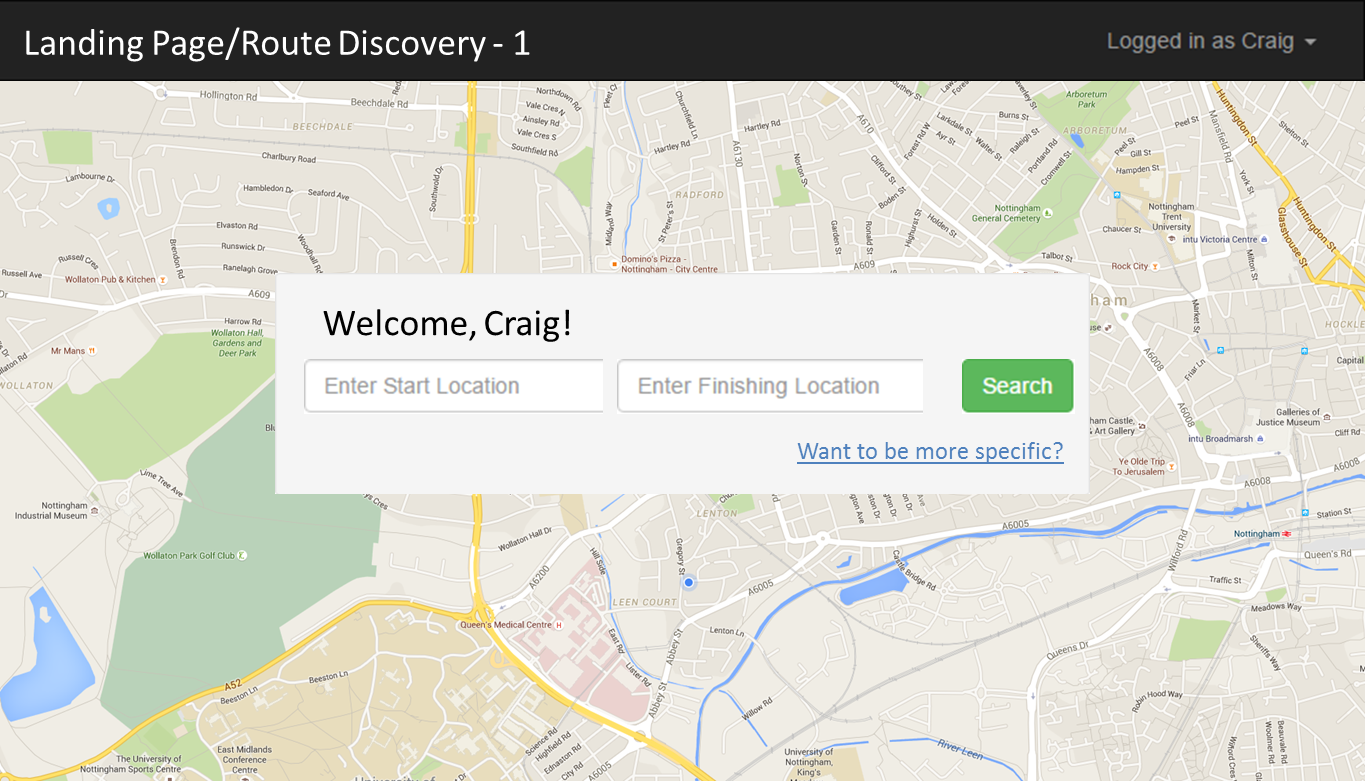
\includegraphics[width=0.8\textwidth]{images/ui-landing-1.png}
	\end{center}
	\vspace{-6mm}
\end{figure}\ \\

\newpage 
\paragraph{Detailed Search Design}\ \\
Compared to the first design, this design is less minimalistic, as it has all searchable fields visible on the page at once. There is an issue here that the users see this large number of fields and are intimidated and exit the application. To combat this it has been placed on the left hand side - this allows the users to view the site from left to right, as would be expected, and thus more comforting. This also gives the map a large interrupted view, which is aesthetically pleasing to look at.\ \\
\ \\
The design ties in well with design 2 of the route listing page, which displays all the search results in the left hand side of the screen. This would mean that the UI could update slightly to display the search results, and the route listing page would be visible without requiring a new page to be loaded - speeding up the process.
\begin{figure}[!ht]
	\begin{center}
		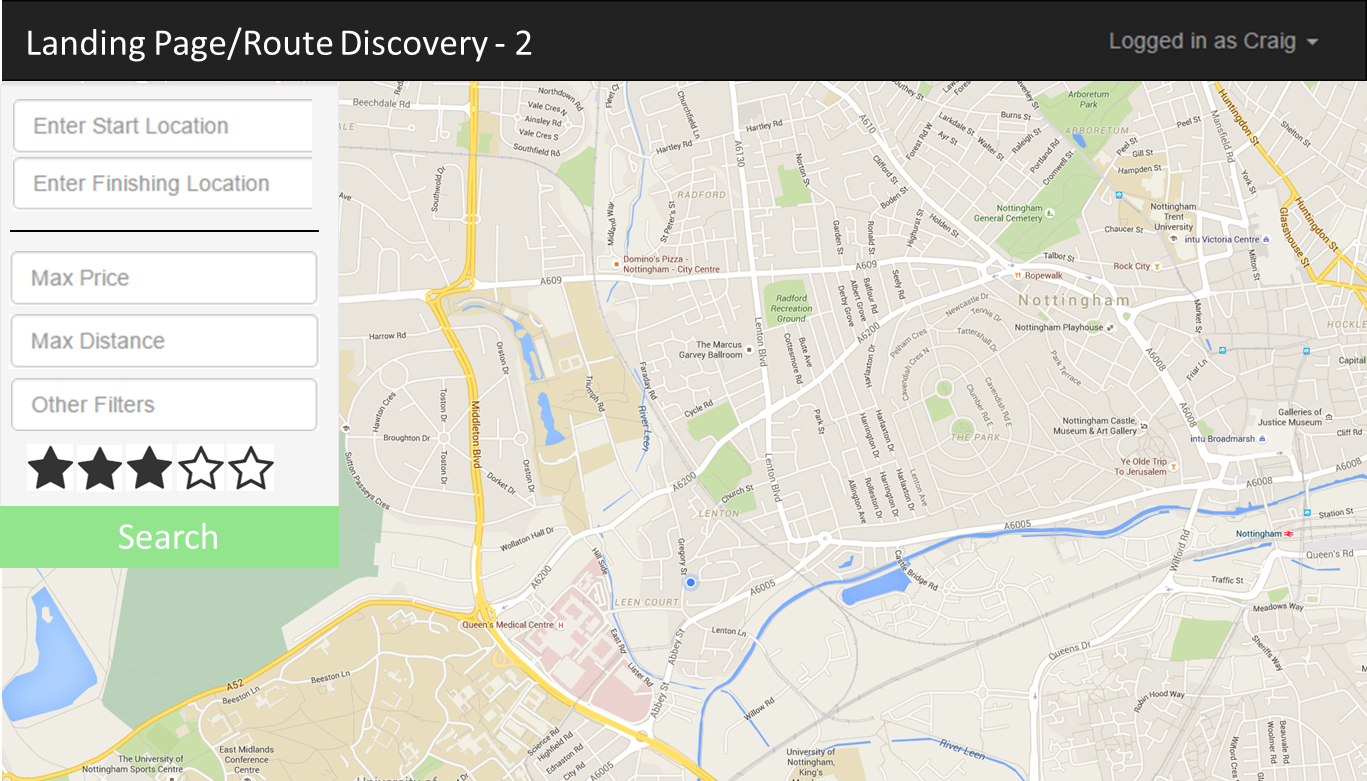
\includegraphics[width=0.70\textwidth]{images/ui-landing-2.png}
	\end{center}
	\vspace{-9mm}
\end{figure}

\paragraph{Modern Design}\ \\
The third design was slightly more unique, and would be supplemented with CSS animations to make it more modern looking. The aim of this design is to look modern, and split up data entry, so that the user is not overwhelmed. They are able to enter the start and end location and then, based on that, enter filtering options. This help to reduce the individual cognitive load of each of the steps, but means that there are more steps to go through until the user reaches the route detail page. Another issue to consider is that the user may be initially lured in by only requiring to enter two fields, but feel cheated when they are then presented with several more.


\begin{figure}[!ht]
	\begin{center}
		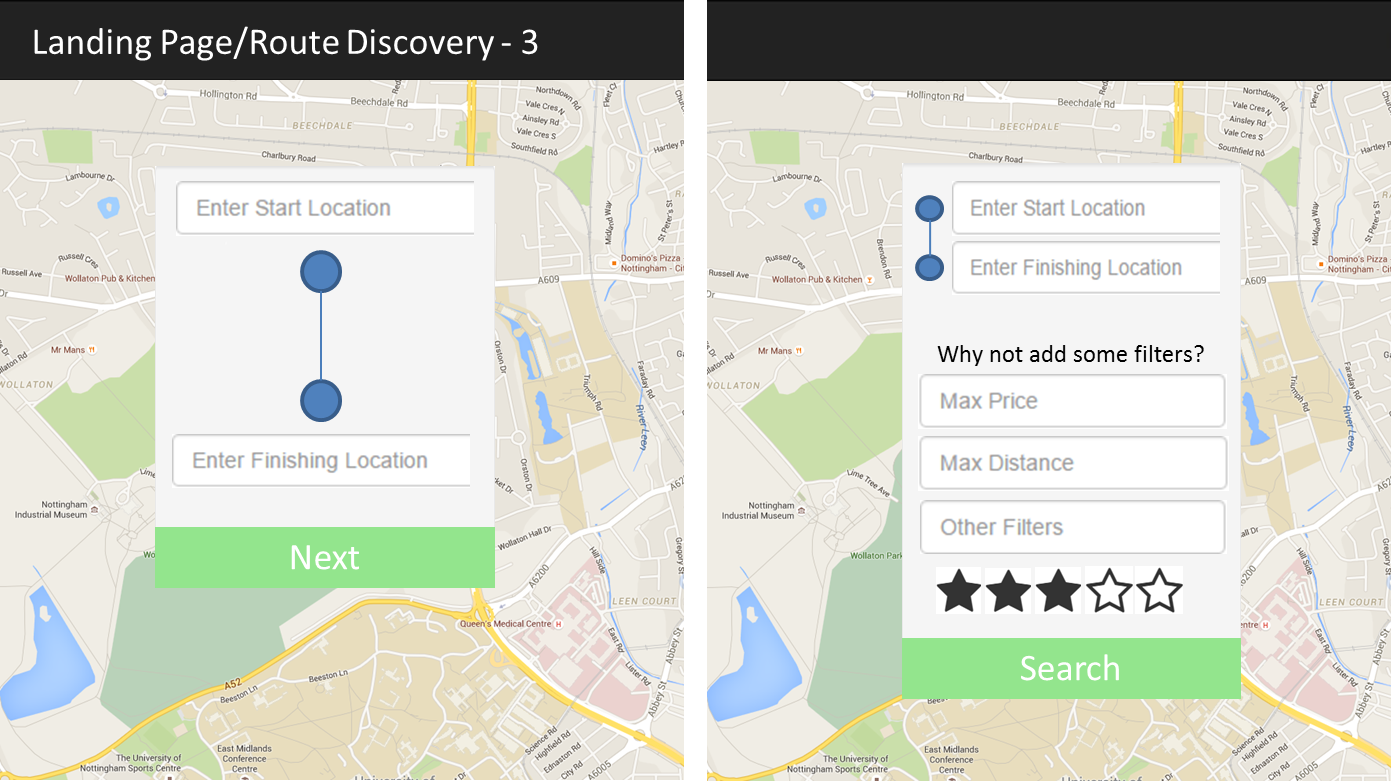
\includegraphics[width=0.70\textwidth]{images/ui-landing-3.png}
	\end{center}
	\vspace{-10mm}
\end{figure}


\newpage 

\subsection{The Route Listing Page (RLP)}
The purpose of the route listing page was to display all of the routes that satisfied the user's search criteria, from the route discovery page. It is important that as many routes are shown as possible (to increase diversity, and the number of choices available), and that they are displayed in a clear, and easy to digest format. (FR 1).

\paragraph{Two Column Design}\ \\
The first design sports a large map, and a clear separation between the map and the list of routes. This dual layout meant that users could find a route in multiple ways - they could select a route from the list that caught their eye, or they could select a route that was close to a specific location (from the map view). This freedom helps to prevent the user becoming confused, or frustrated, when they cannot achieve their goal. The map view is also useful for identifying related routes, which could entice the user to visit the application again later.\ \\
\ \\
The main drawback of this design is the vast quantity of information displayed to the user at once. There is the list, which is a large amount of textual data, combined with the map, which is a large amount of image data. This vast choice could overwhelm the user, and they may not be able to pinpoint any route the would like to traverse. There is also a potential problem in that, if there are a huge number of routes, the map could become cluttered and unusable.
\begin{figure}[!ht]
\vspace{6mm}
	\begin{center}
		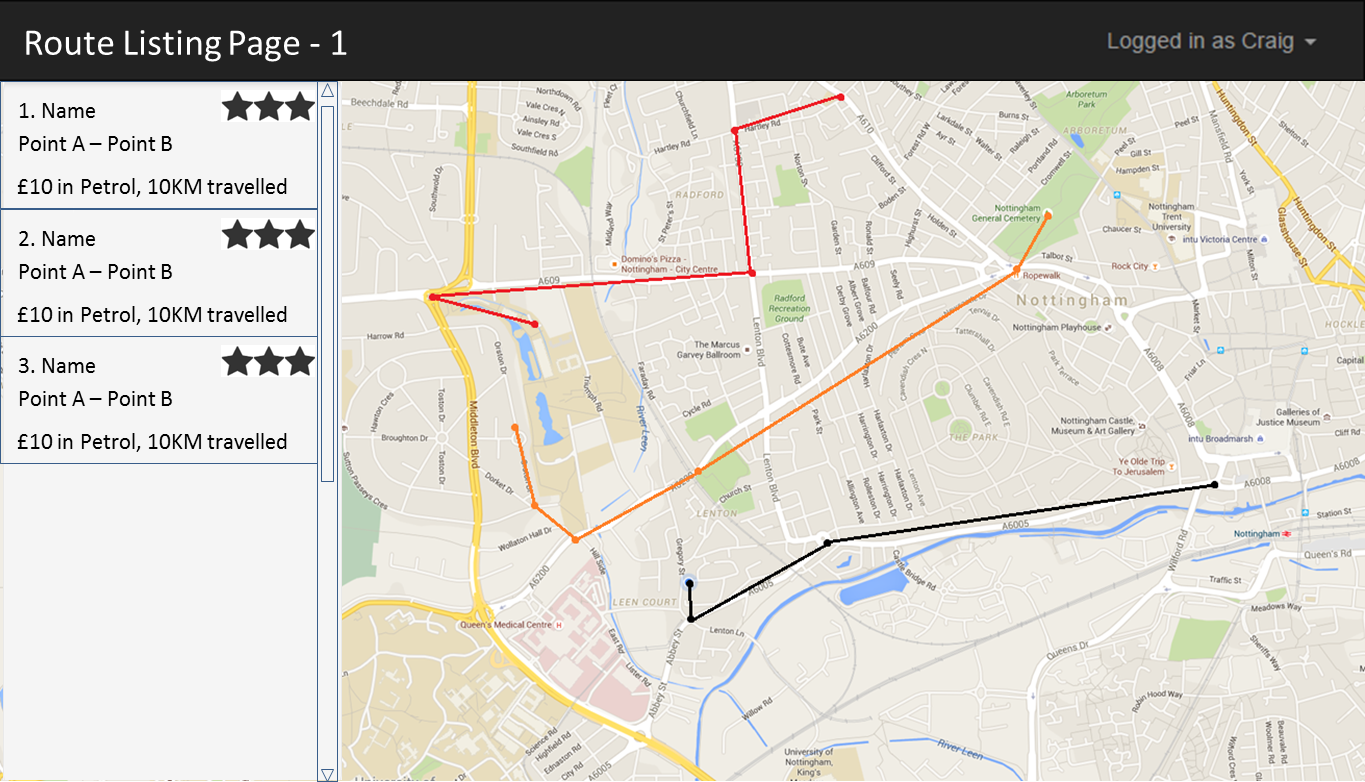
\includegraphics[width=0.85\textwidth]{images/ui-rlp-1.png}
	\end{center}
	\vspace{-6mm}
\end{figure}

\newpage 
\paragraph{Minimalist Design}\ \\
This design also featured a large map. In fact, this map was even larger than the map present in the first design. This is because this design did not feature a textual listing of the routes available. Instead, it relied solely on the graphical display of the routes to provide the user interaction. This makes the design very minimalistic and simple, but a novice user could easily be confused as to what they had to do at this step, and give up (admittedly it would not be too difficult to add a simple pop-up that explained the page). The terms that were used whilst searching for these routes are displayed as pills at the top of the page, so the user can identify if they have made any mistakes in their search.

\begin{figure}[!ht]
	\begin{center}
		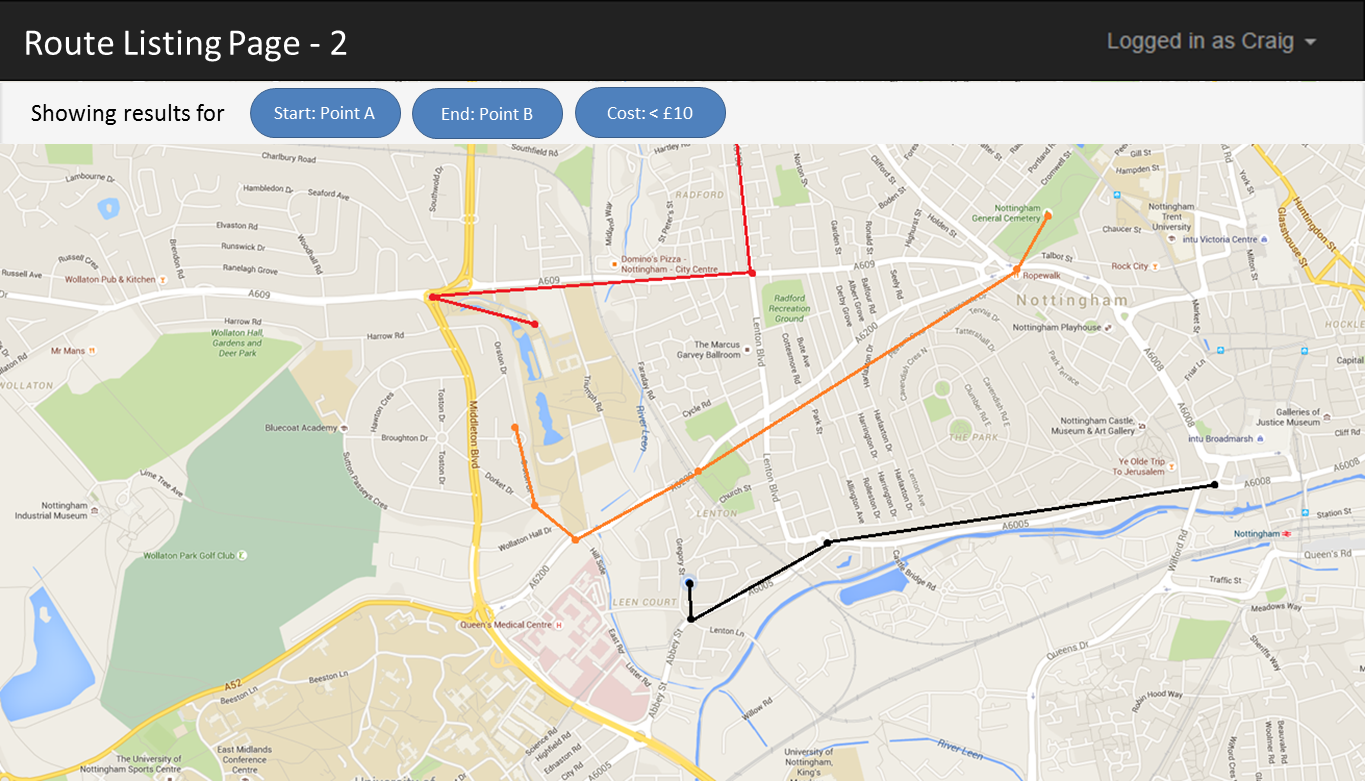
\includegraphics[width=0.7\textwidth]{images/ui-rlp-2.png}
	\end{center}
	\vspace{-9mm}
\end{figure}

\paragraph{Map-less Design}\ \\
The final design for the route listing page differed from the others in that it didn't display one large map with all of the routes. Instead, it opted to show each of the routes individually on their own map. This meant that each one could be considered separately, and the user wasn't overwhelmed with a huge variety of routes at once. The other key feature of this design was the inclusion of the discovery UI. This meant that the user could search again directly from this page, instead of needing to go back to the landing page, like that would in the other designs.\ \\
\ \\
The main problem of this design is that, if there are many routes, those at the bottom of the list would never be seen, as the user probably would not scroll that far. To combat this, some randomness could be added to the algorithm that determines the order of the routes. However, this would also encourage submissions to be of a higher quality, so that they were not placed far down in the list.
\begin{figure}[!ht]
	\begin{center}
		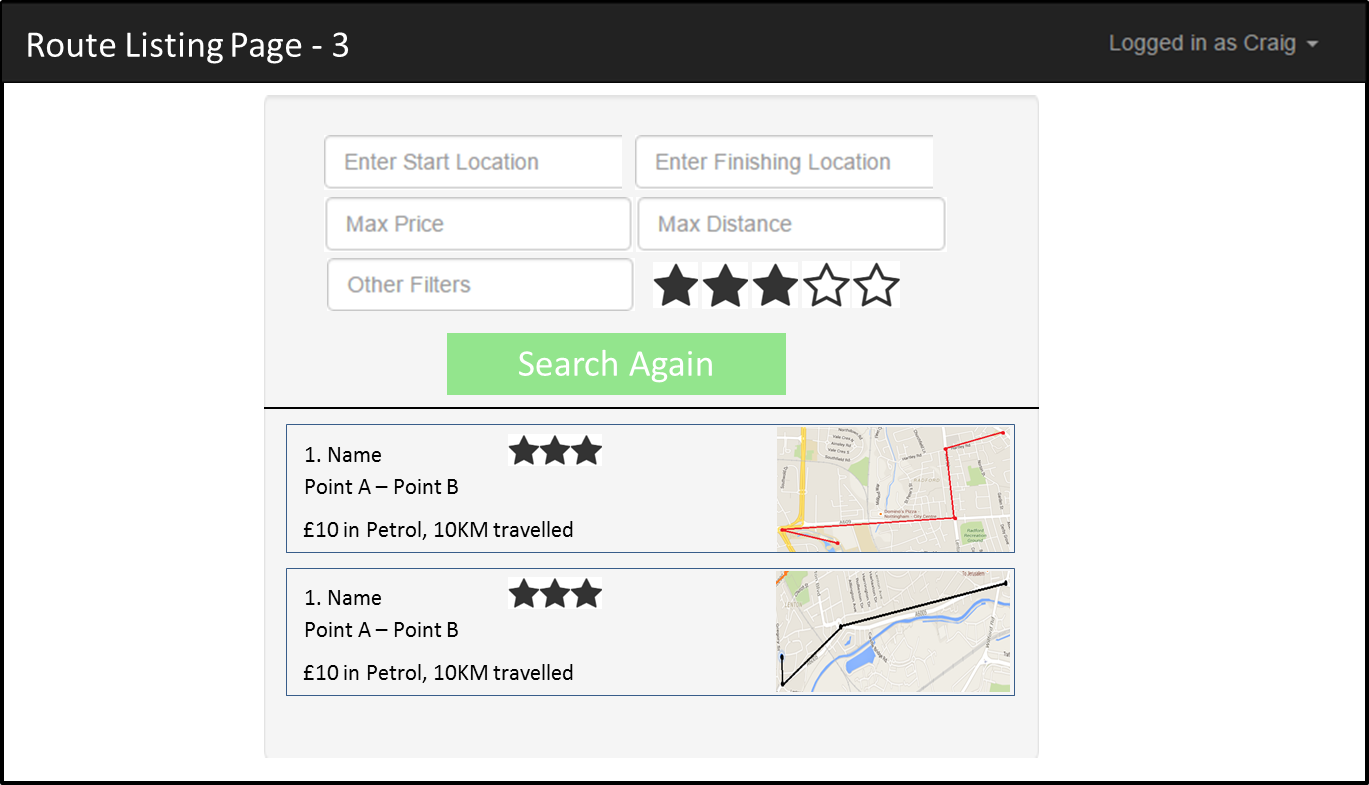
\includegraphics[width=0.7\textwidth]{images/ui-rlp-3.png}
	\end{center}
	\vspace{-9mm}
\end{figure}

\subsection{The Route Detail Page (RDP)}
The purpose of the route detail page is to display both the route, and meta information about it. It is important that information on this page is easily accessible, so users can make informed decisions as to whether or not they wish to travel a route or not. Users will also be able to see, and leave comments on routes from this page. Extra features will be available to admin users, such as comment moderation, and route management (FR 3, 3.1, 3.2, 3.3, 5.2, 5.2.1, 5.2.2, 5.3, 5.3.1, 5.3.2, 6).

\paragraph{Left-heavy Design}\ \\
The first design takes a two column layout, with key information on the left, and a map of the route on the right. This means the user can see important information, like cost and distance, immediately and then investigate further if they so wish. However, as a result of this, the left side is very densely populated, leaving large gaps on the right hand side, and potentially scaring users away due to an information overload.
\begin{figure}[!ht]
	\begin{center}
		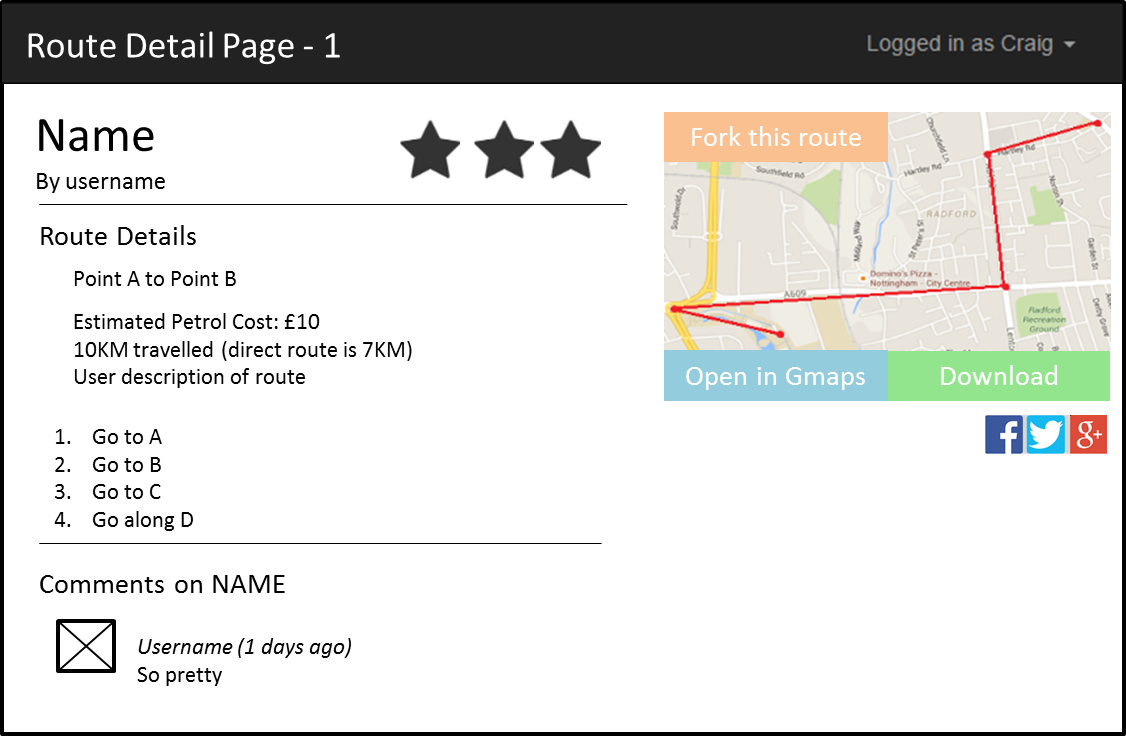
\includegraphics[width=0.5\textwidth]{images/ui-detail-1.png}
	\end{center}
	\vspace{-6mm}
\end{figure}

\paragraph{Two Column Design}\ \\
The second design also uses a two column layout, but utilises the space better. The map and it's details are on the left, so that users can see what they will be doing and where they will be going. If they are interested in the route, they can look to the right to see all the other information, as well as comments from other users. This prevents the user from being overwhelmed by too much information, but allows them to discover more if they wish.
\begin{figure}[!ht]
	\begin{center}
		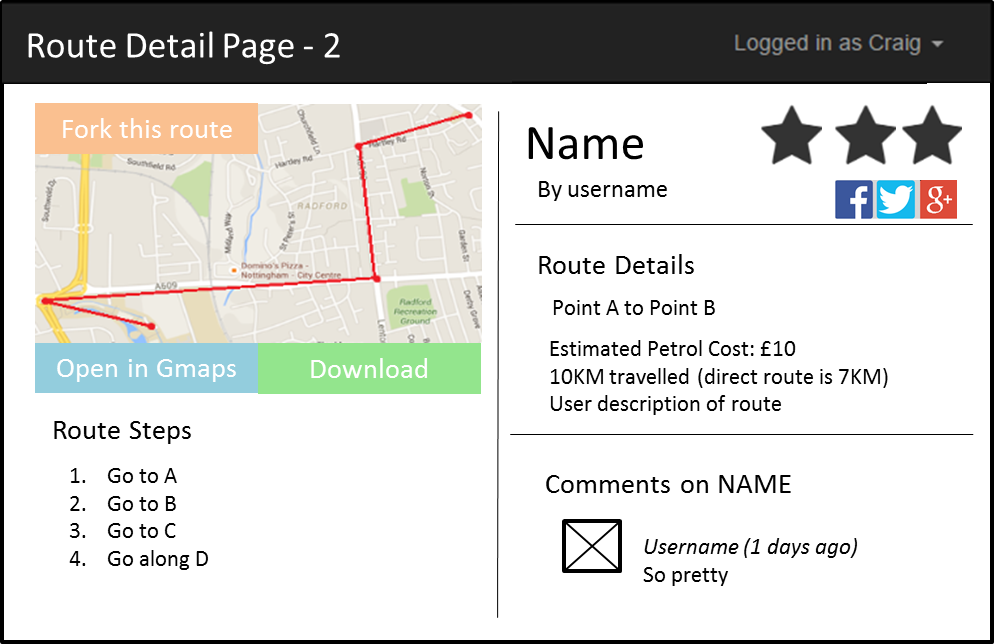
\includegraphics[width=0.5\textwidth]{images/ui-detail-2.png}
	\end{center}
	\vspace{-12mm}
\end{figure}


\newpage 
\paragraph{Map Centric Design}\ \\
The final design for the route detail page was very much focused on the visualization of the route. The only information displayed on the page was the name and rating of the map, and the route itself. The use could click on individual points on the route to get information about it (like a description and how long into the journey this point is). If they wished to see details about the route itself, there was a button for this on the side, which would bring up a side-bar element contain this information. They could also click the ``See comments'', and ``Fork this route'' buttons to display those features in the sidebar. This is a clean, minimalistic design, but could have issues with where users may not know how to see key route information and other user's comments.
\begin{figure}[!ht]
	\begin{center}
		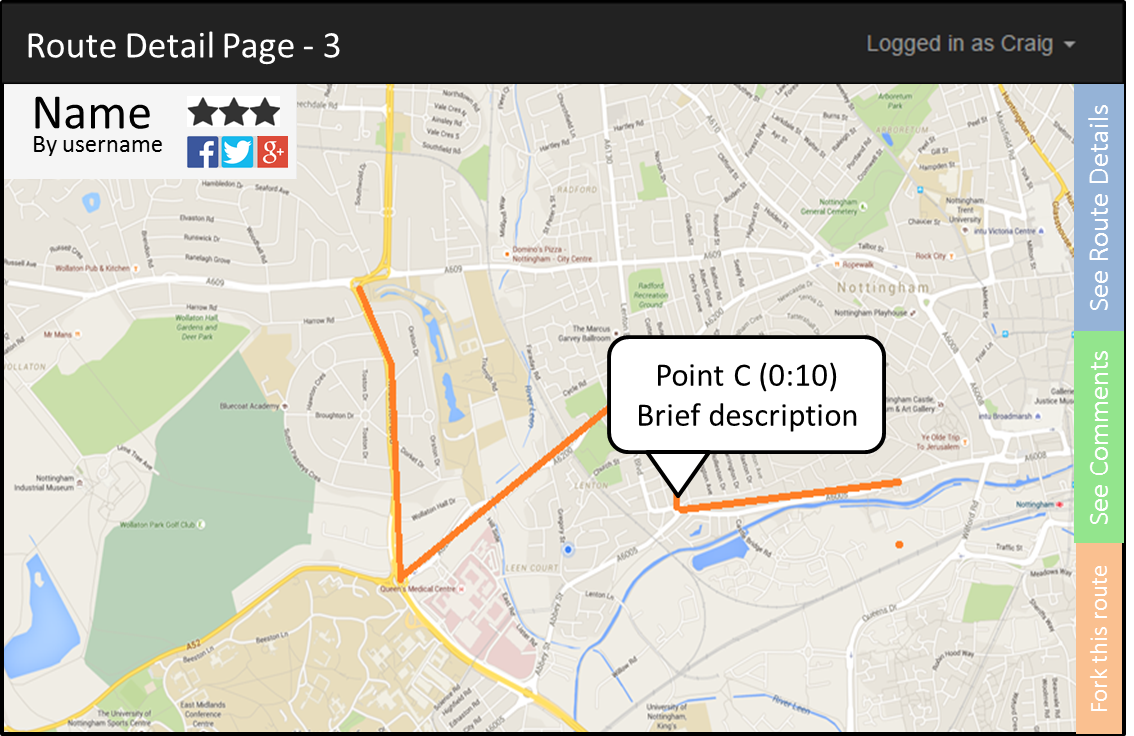
\includegraphics[width=0.7\textwidth]{images/ui-detail-3.png}
	\end{center}
	\vspace{-6mm}
\end{figure}

\subsection{The Route Creation Page (RCP)}
The route creation page was used to specify points of interest, and combine them into a route. The user can use a map to click on locations to add them as points of interest, and they will be automatically connected. The user is free to add points, delete points, and edit the order of points as they wish. Once the route is complete, the user can submit it, allowing them to specify a name, the privacy settings, and a description (FR 2, 2.1, 2.2, 8).


\begin{figure}[!ht]
\centering
	\begin{minipage}{.49\textwidth}
		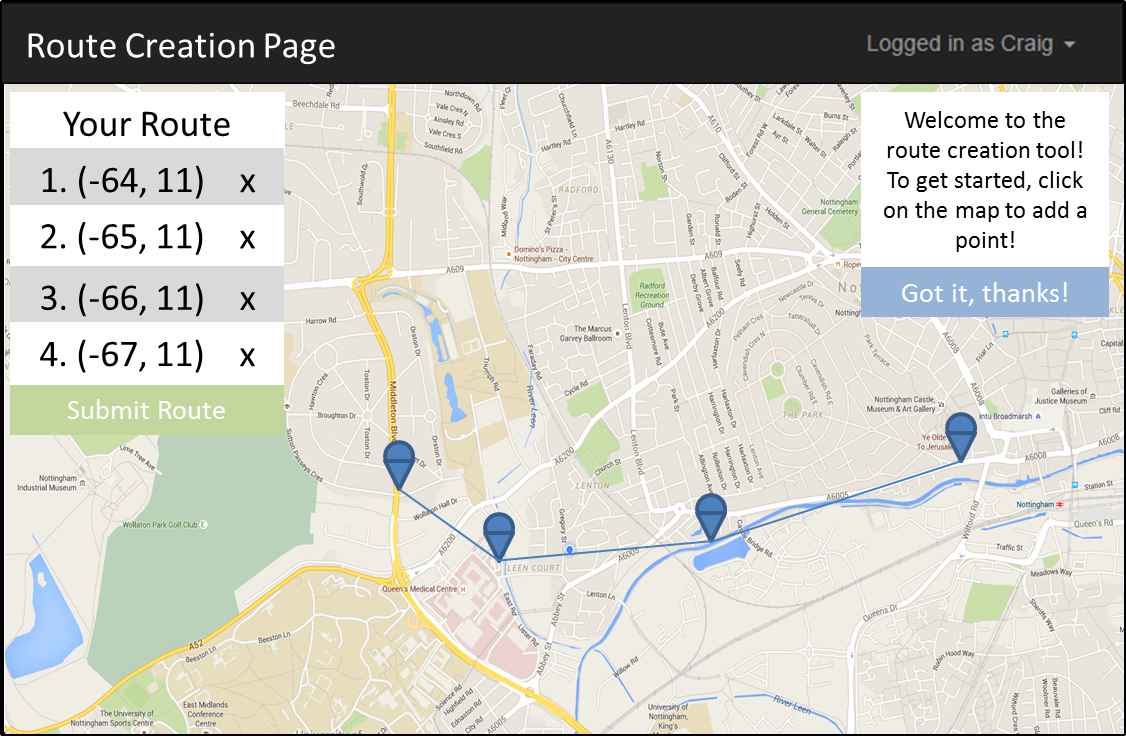
\includegraphics[width=0.99\textwidth]{images/ui-rcp-1.png}
	\end{minipage}
	\begin{minipage}{.49\textwidth}
	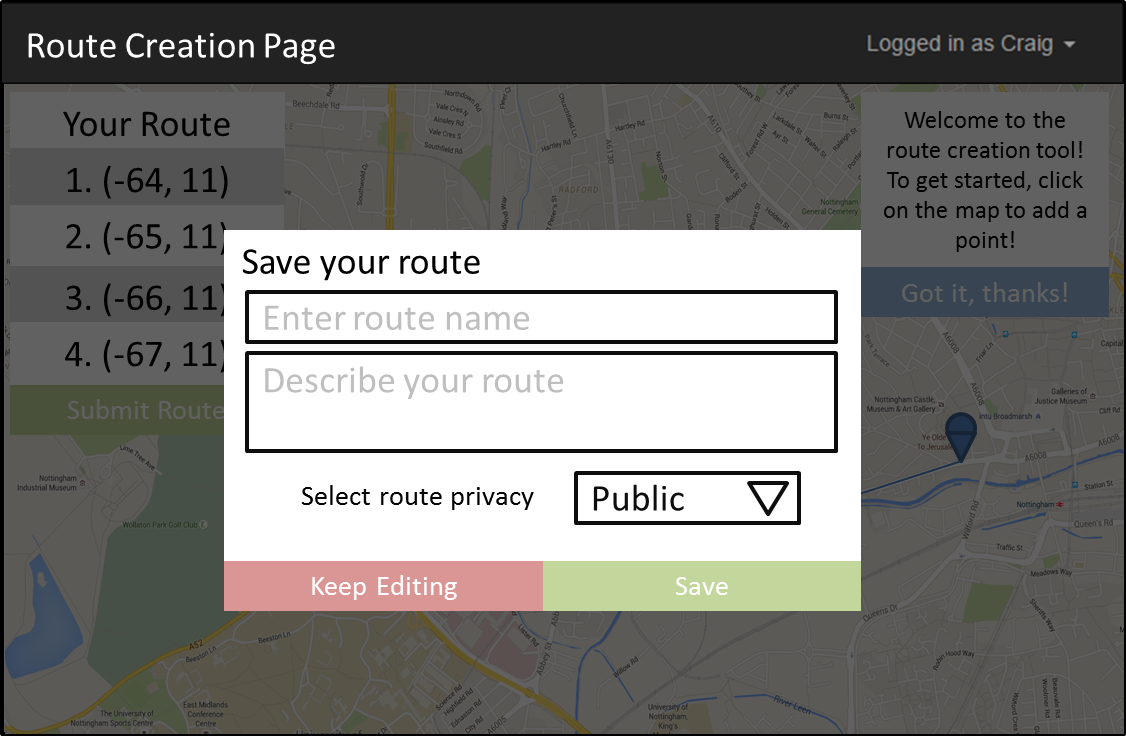
\includegraphics[width=0.99\textwidth]{images/ui-rcp-2.png}

	\end{minipage}
\end{figure}


\newpage 
\subsection{Generic Page Designs}
\label{subsec:gpd}
This section details the ``generic'' pages of the application - those that are mostly form based, and do not require a large amount of design consideration. It includes a basic design, annotated with the functional requirements of the system. 


\subsubsection{Login Page}
The login page is as simple as possible, as to not detract from the purpose of the page. It provides the ability to log in to the user's account (FR 9), by entering their username and password, and the ability to go to the sign up page, if they do not have an account (FR 4). There will be a large scenic picture in the background, as this will increase the aesthetic of the page, fit with the team of the application, and hopefully trigger some emotional response from the user.
\begin{figure}[!ht]
	\begin{center}
		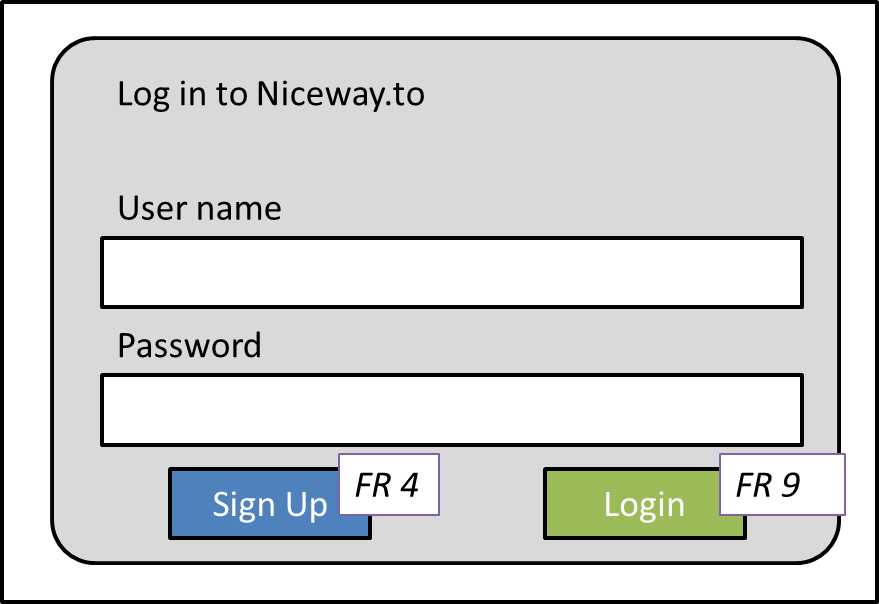
\includegraphics[width=0.45\textwidth]{images/ui-login.png}
	\end{center}
	\vspace{-6mm}
\end{figure}

\subsubsection{Sign Up Page}
Almost exactly like the login page, the sign up page is a very simple form allowing for users to enter in their details and create an account (FR 4), without being distracted by others elements on the page. This will actually be present on the same page as the login page, so the user is not required to navigate to another page simply to sign up, instead they can do it from the log in page, which will speed of the process of creating their account.
\begin{figure}[!ht]
	\begin{center}
		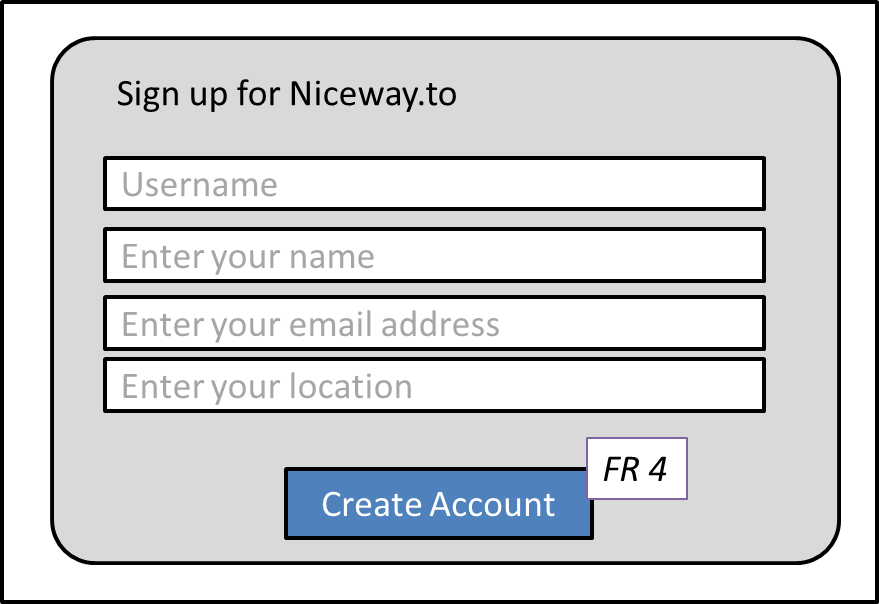
\includegraphics[width=0.45\textwidth]{images/ui-signup.png}
	\end{center}
	\vspace{-6mm}
\end{figure}

\newpage 
\subsubsection{Account Page - My Routes}
The ``My Routes'' page is used to display and manage all of the routes that a user has submitted, or forked, with the ability to add a new route (FR 9.2, 2, 2.1, 2.2). It will be on a generic ``My Account'' page, which means all similar actions are clustered together, and the user will know exactly where to navigate to perform any given task. On this particular page, the user's routes will be listed, along with key information (name, start location, end location, and privacy), with the ability to edit these settings, edit the route, delete the route, or export/download the route (FR 6). For users with many routes, a paginated view will be displayed.
\begin{figure}[!ht]
	\begin{center}
		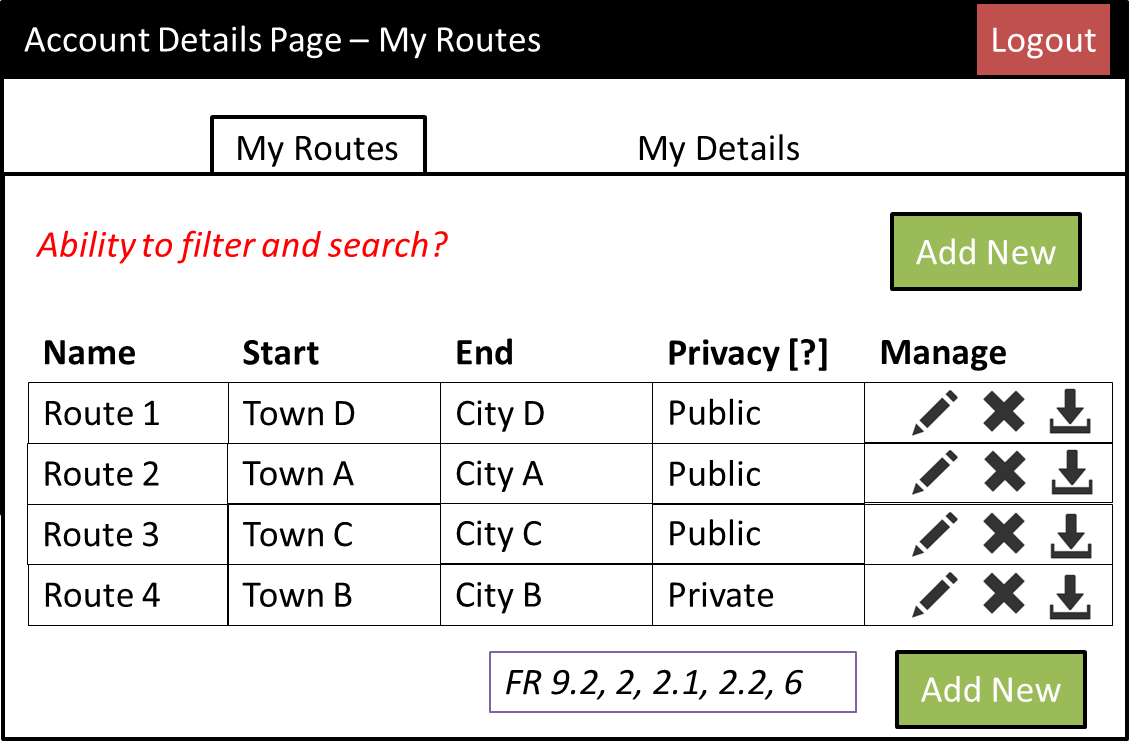
\includegraphics[width=0.6\textwidth]{images/ui-myroutes.png}
	\end{center}
	\vspace{-6mm}
\end{figure}\ \\

\subsubsection{Account Page - My Details}
Similarly to the ``My Routes'' page, the ``My Details'' page will be accessible from the generic ``My Account'' page. This page will simply display all of the user's data (excluding their password), with the ability to modify and update them (FR 4, 9.1). The page will be split into sections, so that similar data is situated together, for instance, the personal details section, and the update password section. This is so that users can jump to the exact functionality they require, rather than having to look through a large list of possible options. Users will also be given the ability to close their accounts on this page. 
\begin{figure}[!ht]
	\begin{center}
		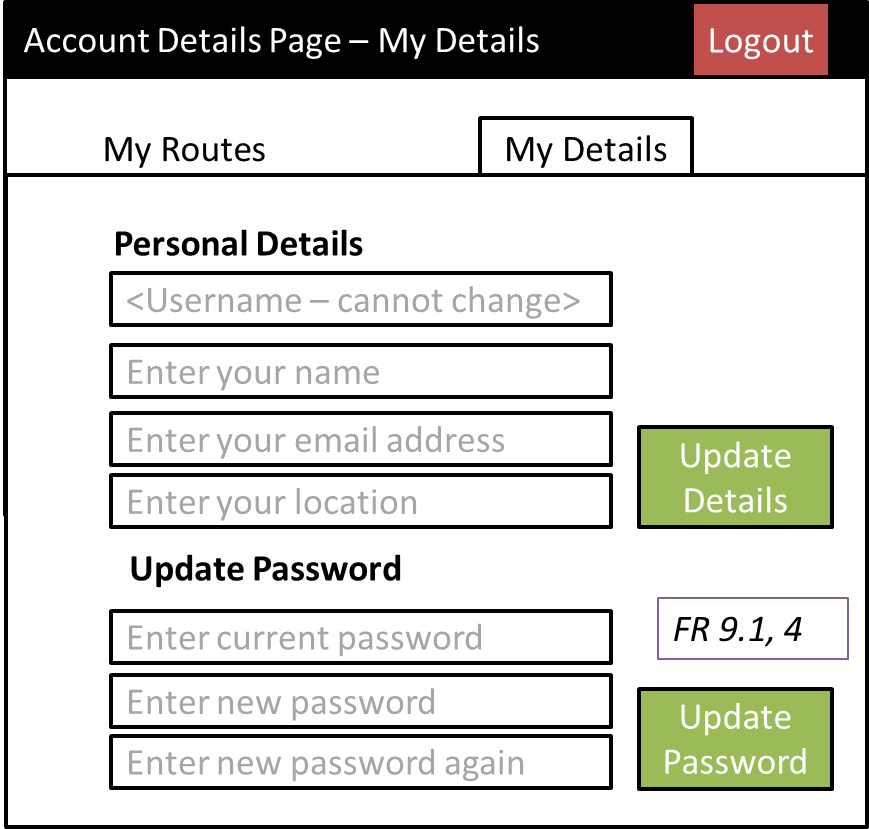
\includegraphics[width=0.5\textwidth]{images/ui-mydetails.png}
	\end{center}
	\vspace{-12mm}
\end{figure}

\subsubsection{Account Page - Administration}
The final generic page is the administration page, which like the previous two pages, will be located in the generic ``My Account'' page. This page will only be viewable and accessible to users with administrative privileges on Niceway.to. The page will provide multiple tools that the administrators can use to maintain the site, and manage users. The keys features are: a user search tool, with the ability to edit user details, delete users, ban them and shadow ban them \footnote{Allow the user to keep using the site, but none of their comments or routes will be visible to other users}; an account creation tool, with the ability to create new accounts on the site; an announcements tool, allowing the admin to post announcements to the site (as well as email users); and some server management tools, including making backups, reauthorizing active sessions, and locking the site. Similarly to the accounts page, these will be split up, so they are easier to see as distinct tools. 
\begin{figure}[!ht]
	\begin{center}
		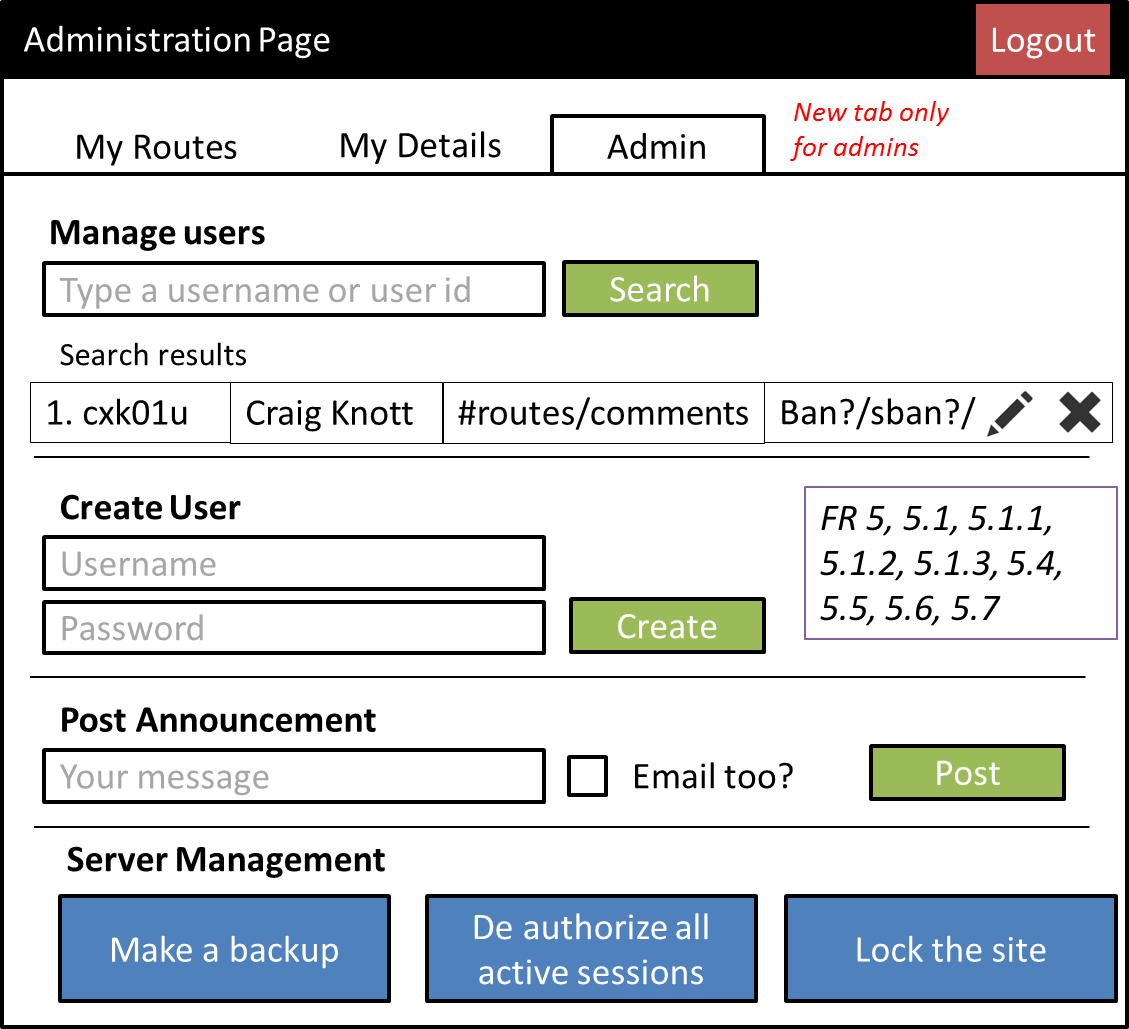
\includegraphics[width=0.7\textwidth]{images/ui-admin.png}
	\end{center}
	\vspace{-6mm}
\end{figure}


 
\subsection{User Flow Diagram}
 This diagram shows the expected user flow through the application. All user journey's will begin on the landing page, which also serves as the route discovery page. From here, users are free to search for routes, and experience the application, without every having the need to log in. They will have the ability to sign in, or sign up, from multiple locations, however, to increase the likelihood of them doing so (for instance, in the navigation bar of every page, and on the route detail page, prompting them to sign up so they can comment). Once a user has searched for a route, they will be taken to the route detail page, which will give users all the necessary information so that they can complete the route.\ \\
 \ \\
 If users wish to log in, or sign up, they will then be able to access their profile page, where they can see their submitted (and forked) routes, and modify their personal information. This is also where administrators will be able to access administrative tools for the management of the application. \ \\
 \ \\
The final feature available is route creator, which the user can access from the landing page (with the ``submit new route'' button), or from the ``My Routes'' section of the profile page. This means that it is extremely easy for the user to submit content to the site, as they are confronted with this option as soon as they visit the site, and whenever they view their other submissions.
 
 \begin{figure}[!ht]
 \begin{center}
 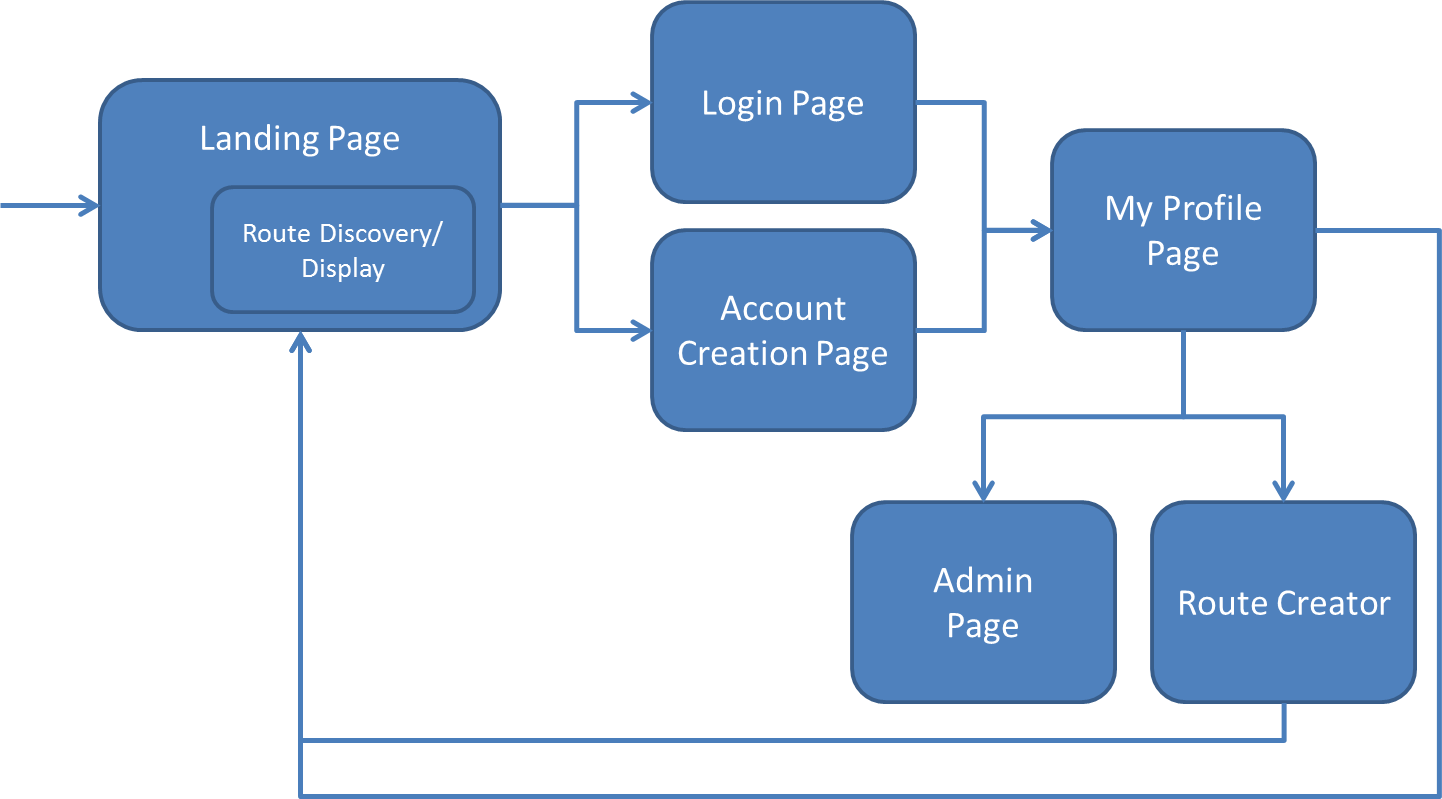
\includegraphics[width=0.7\textwidth]{images/flow.png}
 \end{center}
 \vspace{-6mm}
 \end{figure}
